% This are the basic setting, just leave it
\documentclass[12pt, a4paper, oneside]{report}
\usepackage{amsmath, amsthm, amssymb, graphicx, setspace, newtxtext, listings, subcaption, geometry, multicol}
\usepackage[bookmarks=true, colorlinks, citecolor=blue, linkcolor=black]{hyperref}

\lstset{
  language=R,
  basicstyle=\ttfamily,
  keywordstyle=\color{blue},
}

\geometry{
  top=3cm,
  bottom=3cm,
  left=2cm,
  right=2cm,
}

% This this the title, arthur, and date
% remember to change our name to official name and add email later
\title{ECS132 Term Project Report}
\author{Jonathan Tran\\Alex Din\\Haosen Cao}
\date{\today}

% chktex 36

% Google Doc link
% https://docs.google.com/document/d/1c2Lg5Y1ekLZNBOz9qw190xJkgW0L_A6-DEsg0y5Ebts/edit




% This is the actual content of the report
\begin{document}
\maketitle
\tableofcontents
\newpage







\chapter*{Introduction}
\addcontentsline{toc}{chapter}{Introduction}
In this report we will find and analyze real world data, using proper families of continuous distribution families to present the data with calculations and codes. 
Specifically, this for the four families of continuous distribution families, we will use:

\lstinline{weight} column in \lstinline{national.longitudinal.survey.rda} under \lstinline{fairml} directory to model normal family of distribution.

\lstinline{PRECTOT} column in \lstinline{weatherTS.RData} under \lstinline{qeML} directory to model exponential family of distribution.

\lstinline{GPA} column in \lstinline{lawschoolbrief.RData} under \lstinline{EDFfair} directory to model beta family of distribution.

\lstinline{Age} column in \lstinline{AdultFinal.RData} under \lstinline{EDFfair} directory to model gamma family of distribution.

\newpage





\chapter*{Analysis}
\addcontentsline{toc}{chapter}{Analysis}
\newpage





\newpage
\section*{Normal}
\addcontentsline{toc}{section}{Normal}
To model the normal family of distributions we decided to base our model on the weight column of the national.longitudinal.survey data, which contains data of 4908 individuals' statistics like age, race, height, and weight. The weight is distributed in the range from 87 to 325. When we plotted the histogram, most of the data are in the range from 100 to 200, and as we go to the left or right of that, the number of points decreases. But most importantly the data looked similar to a bell curve.

%expHistDefault, %expDensityDefault
\begin{figure}[h]
  \centering
  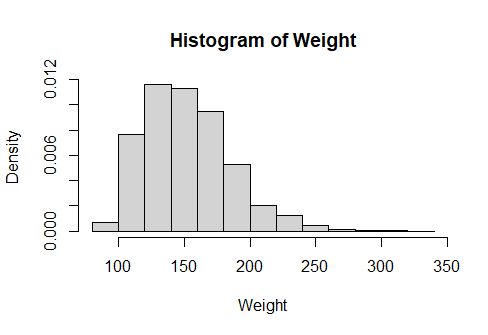
\includegraphics[width=0.7\linewidth]{normHist.png}
\end{figure}

\begin{figure}[h]
  \centering
  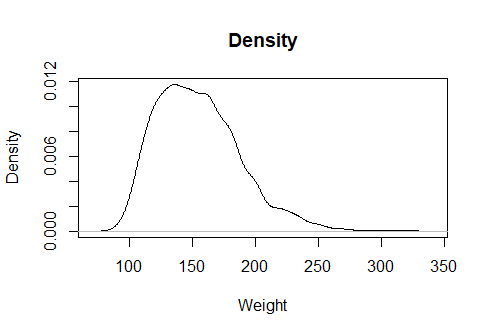
\includegraphics[width=0.7\linewidth]{normDensity.png}
\end{figure}

\newpage
The normal family of distributions has two parameters, mean and standard deviation. We are assuming that the weights in this dataset can be modeled with a normal distribution. Therefore we use two methods to find estimates for the mean and standard deviation parameters, which we will call \(M\) and \(SD\), respectively.

For maximum likelihood, we used R's \lstinline{mle()} function to find \(M\) and \(SD\), which takes a negative log-likelihood function. While the likelihood function is the product of density functions on the given data, the log-likelihood is the sum of the logarithm of those density functions. Therefore we use this line as our negative log-likelihood function:

\begin{lstlisting}
loglik <- sum(dnorm(weights, M, SD, log = TRUE))
\end{lstlisting}

Where weights is our weight data, and \(M\) and \(SD\) are our parameter estimates. Plugging this into the \lstinline{mle()} function gives us \(M = 154.5827\) and \(SD = 33.18112\).

The method of moments for a normal distribution is relatively simple. The two parameters of the normal distribution are the mean and standard deviation, which we can generate estimates for using our sample data directly from R. \(M\) is just \(\bar{A}\), our sample mean from calling \(mean(weights)\), and \(SD\) is just \(\sqrt{S^2}\) which can be given by calling \(sqrt(var(weights))\). The difference between using \(S^2\) and \(s^2\) is negligible. Using this method, we get \(M = 154.5827\) and \(SD = 33.18453\).

\begin{figure}[h]
  \centering
  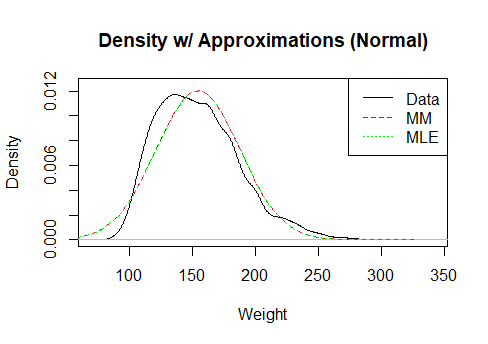
\includegraphics[width=\linewidth]{normDensityA.png}
\end{figure}

\newpage
We would say that the normal family is a suitable estimator for the weights in this dataset. A normal distribution, according to the central limit theorem, is what results from a set of summations of random variables. The weight of a person can be thought of as a sum of the various parts of their body, whose sizes can be thought of as random. 
However, based on the graph, which has a slightly steeper slope on the left side than on the right, it can be argued that a gamma distribution would better model this data. 

\begin{figure}[h]
  \centering
  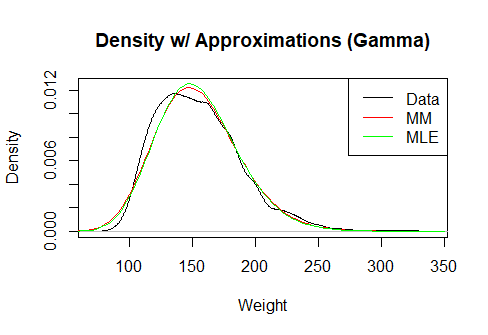
\includegraphics[width=\linewidth]{normButGamma.png}
\end{figure}

And from the graph, we must concede that the gamma family may model this data better than the normal family. But if the central limit theorem says that sums of random variables look normal, and the gamma distribution is a sum of exponentially distributed random variables, it’s no wonder that the graphs look pretty similar. If we’re summing a large enough number of exponential variables, it’s possible that the gamma distribution could converge to a normal distribution. From this line of thinking, the normal and gamma distribution are likely both good estimators for the weights in the dataset.












\newpage
\section*{Exponential}
\addcontentsline{toc}{section}{Exponential}
To model the exponential family of distributions we decided to base our model on the PRECTOT column of the weatherTS data, which looks like it took weather data from Eastern Australia for 10 years (1985--1995).
Of this data, the one we were most interested in was the PRECTOT column, which we interpreted as the total precipitation on a given day.
When we plotted the histogram, the data was heavily skewed left, tapering off more to the right, which resembled that of an exponential graph.
The most important thing was that the peak of the data was at \(x = 0\), which is where exponential graphs peak.

%expHistDefault, %expDensityDefault
\begin{figure}[h]
  \centering
  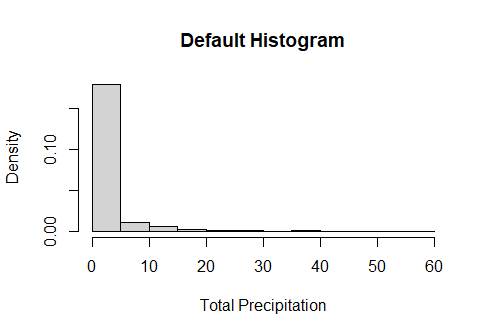
\includegraphics[width=0.7\linewidth]{expHistDefault.png}
\end{figure}

\begin{figure}[h]
  \centering
  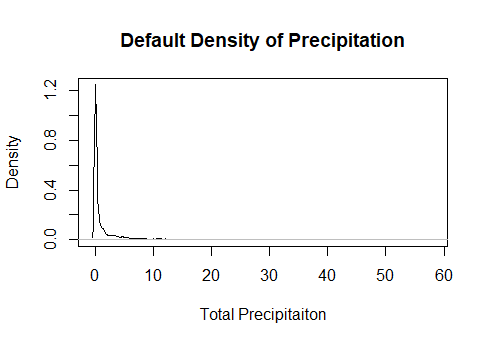
\includegraphics[width=0.7\linewidth]{expDensityDefault.png}
\end{figure}

\newpage
Just from looking at these graphs, while the density function doesn’t look quite exponential, the histogram definitely does. We will discuss possible reasons why later on. But for now, we will find estimators for the parameters of the exponential family.
The exponential family is a one-parameter family, that being lambda. Using the two methods, we are trying to find an estimator for lambda, which will be referred to as \(L\).
We use this line of code to get the negative log-likelihood function for our maximum likelihood.

\begin{lstlisting}
loglik <- -sum(dexp(prectot, L, log = TRUE))
\end{lstlisting}

Where prectot is our precipitation data and \(L\) is our estimator for lambda.
Plugging this into the \lstinline{mle()} function we get \(L\) to be 0.5230325.

%newline

Next, for method of moments, we algebra to estimate \(L\).
For a given exponentially distributed variable \(X\), the expected value is given by \(E(X) = \frac{1}{\lambda}\). Assuming the mean of our sample data, \(\bar{A}\), is an unbiased estimator for the true mean of the population data, \(\bar{A} = \frac{1}{L}\), and therefore \(L = \frac{1}{\bar{A}}\).
Plugging this into R we get \(L\) to be 0.5230367.

%newline

Because this is a one-parameter family, we can also derive \(L\) from our sample variance \(s^2\). The variance of an exponentially distributed variable X is given by \(Var(X) = 1 / \lambda^2\). Therefore \(L\) is given by \(L = \sqrt{1 / s^2}\).
With this method, \(L\) is shown to be 0.2002137, which is very different from the other two methods above. From the graphs below, this particular estimate for lambda isn't very good. 

\begin{figure}[h]
  \centering
  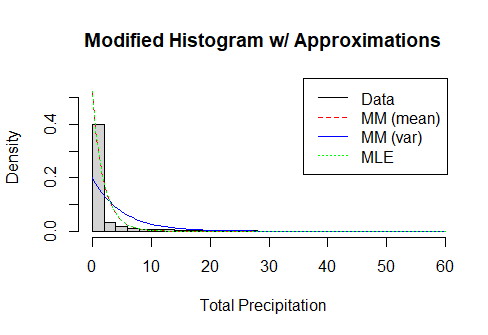
\includegraphics[width=0.7\linewidth]{expHistModifiedA.png}
\end{figure}

\begin{figure}[h]
  \centering
  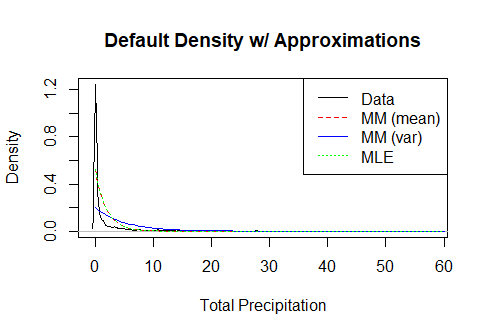
\includegraphics[width=0.7\linewidth]{expDensityDefaultA.png}
\end{figure}

\newpage
It is important to note that our exponential distribution plots don't quite match those of the \lstinline{hist()} or \lstinline{density()} functions on our sample data, at least with their default arguments. These discrepancies can be attributed to a bandwidth that doesn't accurately reflect our sample. 
By decreasing the bandwidth for the \lstinline{density()} function and increasing it for the \lstinline{density()} function, we get graphs that better match our plots.


%expHistModifiedA, %expDensityModifiedA

\begin{figure}[h]
  \centering
  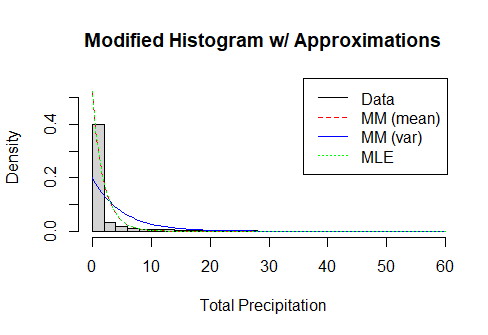
\includegraphics[width=0.7\linewidth]{expHistModifiedA.png}
\end{figure}

\begin{figure}[h]
  \centering
  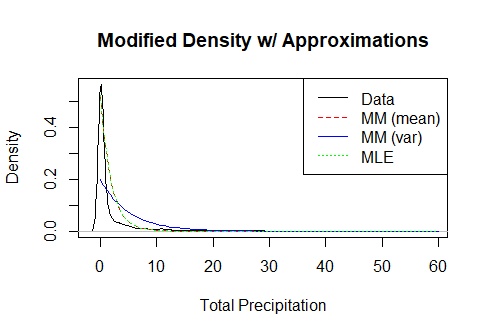
\includegraphics[width=0.7\linewidth]{expDensityModifiedA.png}
\end{figure}

\newpage
The histogram looks good, but the density function is arguably less exponential-looking as a result. Lowering the bandwidth of the density function does make it more exponential, but likely at the cost of being less accurate due to how few points can actually fit into an individual bandwidth. 


\begin{figure}[h]
  \centering
  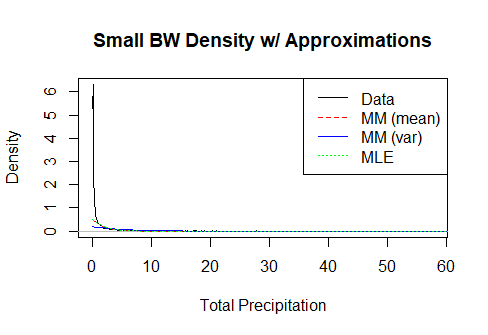
\includegraphics[width=0.7 \linewidth]{expDensitySmallA.png} %expDensitySmallA
\end{figure}


But even with these discrepancies, given our plots of the exponential distribution, we would say this family is a suitable estimator for the total precipitation on a given day in Australia. The exponential distribution is said to be the continuous analog of the geometric distribution. How much precipitation you get in the day is pretty much the same as how long it rains on a given day. And how long it rains in a given day can be thought of as successive failures (the rain continuing) until a single success (the rain stopping), which is like a geometric distribution. Obviously, this is an oversimplification but it shows how an exponential distribution can model the density function of total precipitation.



















\newpage
\section*{Gamma}
\addcontentsline{toc}{section}{Gamma}
To model the gamma family of distributions, we decided to use the age column from the dataset adultfinal, which seems like it contains various data from specifically working individuals. We decided to use age because the histogram we observed was very gamma in nature. It shows a steep increase in the number of people in the beginning and more gradually decreases as we go up in age.

\begin{figure}[h]
  \centering
  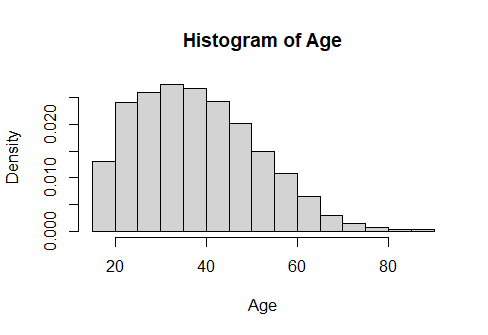
\includegraphics[width=0.7\linewidth]{gammaHist.png}
\end{figure}

\begin{figure}[h]
  \centering
  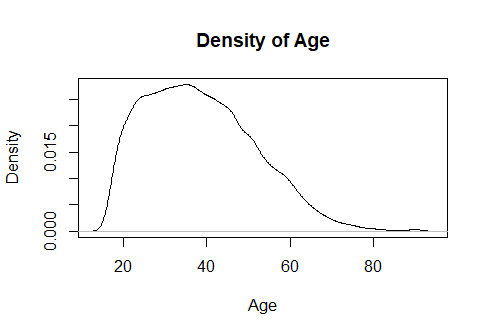
\includegraphics[width=0.7\linewidth]{gammaDensity.png}
\end{figure}

The gamma family can be described as a sum of exponentially distributed random variables. So the gamma family has two parameters, \(lambda\), the same kind as those of the exponential family, and \(r\), the number of exponential variables that are summed together. Assuming that this age data can be modeled with a gamma function, we are trying to find estimates for lambda and \(r\), which will be called \(L\) and \(C\), respectively.
We use this line of code for the maximum likelihood estimator:
\begin{lstlisting}
  loglik <- -sum(dgamma(age, C, L, log = TRUE))
\end{lstlisting}
Pluging this into the \lstinline{mle()} function gives us \(C = 8.596535\) and \(L = 0.2236146\). 
For the method of moments, we again use algebra to find \(C\) and \(L\).

% $E(X) = \frac{r}{\lambda}$

% $\text{Var}(X) = \frac{r}{\lambda^2}$

% $\bar{A} = \frac{C}{L}$

% $C = \bar{A}L$

% $s^2 = \frac{C}{L^2}$

% $s^2 = \frac{A}{L}$

% $L = \frac{A}{s^2}$

\begin{multicols}{2}
  \begin{align*}
  E(X) = \frac{r}{\lambda} \\
  \bar{A} = \frac{C}{L} \\
  C = \bar{A}L \\
  \end{align*}
\columnbreak
  \begin{align*}
  \text{Var}(X) = \frac{r}{\lambda^2} \\
  s^2 = \frac{C}{L^2} \\
  s^2 = \frac{A}{L} \\
  L = \frac{A}{s^2}
  \end{align*}
\end{multicols}



Substituting $s^2$ with $var(age)$ and $\bar{A}$ with $mean(age)$ we get $C = 8.587819$ and $L = 0.2233877$.

\begin{figure}[h]
  \centering
  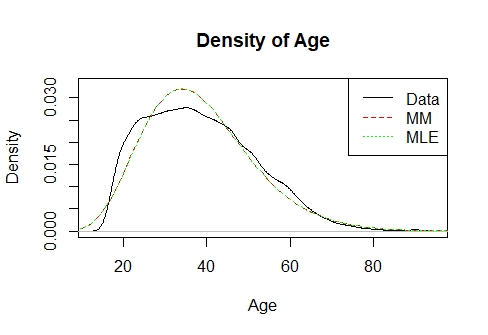
\includegraphics[width=0.7\linewidth]{gammaDensityA.png}
\end{figure}

Judging from the graph, the gamma distribution is a decent estimator for the ages in this dataset. It works especially well for estimating the number of people aged 45 and above. It doesn’t work as well for the rest of the data, but it does the job well enough. In any case, it would be hard to find a distribution family that better fits this data. 
It is important to note that the ages from this sample don’t exactly reflect the age of everyone in a given population. There is some sampling bias here in that the data is only taken from people who have an occupation, and notably, there is no data from anyone aged 16 or below. Because of this, it is hard to justify why this dataset’s age can be described as a gamma-distributed variable since there are a couple of factors going on here.
But in terms of simply fitting the graph of the data, the gamma distribution does the job just fine.









\newpage
\section*{Beta}
\addcontentsline{toc}{section}{Beta}
% https://statproofbook.github.io/P/beta-mome.html
% (8) (9) for alpha and beta










\newpage
\chapter*{Conclusion}
\addcontentsline{toc}{chapter}{Conclusion}
In this report, we model the 4 different dataset with different families of continuous distribution. Specifically, we focused on the normal, exponential, gamma, and beta distribution families. By applying statistical calculation and utilizing programming tool R, we also find estimators for maximum likelihood and method of moments methods.


\end{document}